\LoadClass{tccv}
\newcommand{\mynext}{\\[0.2cm]}
\documentclass{tccv}
\usepackage{graphicx}

\begin{document}


\graphicspath{{wordcloud}}
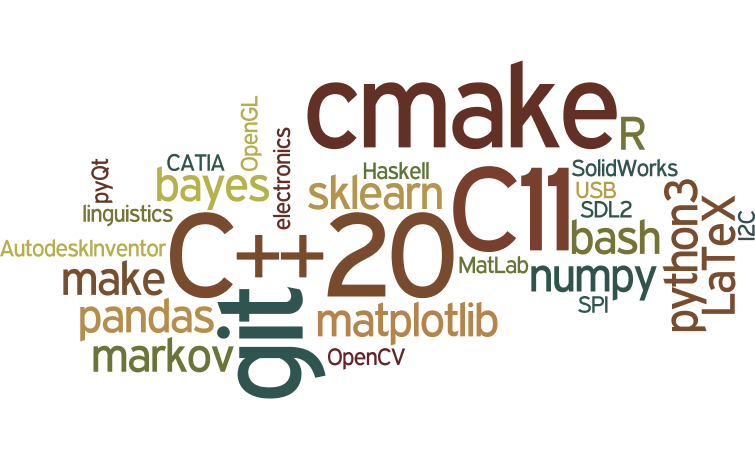
\includegraphics[width=\textwidth]{one}


% engineer!
\part{Miroslav Vitkov}


\section{Technical skills}
\begin{factlist}
\item{Expert}
{
     * C++14 under procedural, object oriented and functional paradigms  \mynext
     * C11 for $\mu$C and ARM applications  \mynext
     * supporting tools git, gitolite, cmake, teamcity
}
\\
\item{Proficient}
{
    * python for ML applications \mynext
    * bash, the LFHS, most standard utilities, security configuration and evaluation, unix sockets  \mynext
    * \LaTeX
}
\\
\item{Experienced}
{
    * R                                            \mynext
    * MatLab                                       \mynext
    * digital and analog hardware design           \mynext
    * USB, I2C, SPI firmware                       \mynext
    * Autodesk Inventor, SolidWorks, CATIA         \mynext
    * SDL2, OpenGL                                 \mynext
    * Haskell                                      \mynext
    * OpenCV                                       \mynext
    * pyQt                                         \mynext
    * Deep learning                                \mynext
    * Computational linguistics
}
\end{factlist}


\section{Communication skills}
\begin{factlist}
\item{Bulgarian}{C2: Native speaker}
\item{English}{C2: Fluent (Cambridge CPE)}
\item{German}{A1: Basic}
\end{factlist}


\personal
    {Druzhba-2, Sofia, Bulgaria}
    {0895 735 164}
    {sir.vorac@gmail.com}


\section{Education}
\begin{yearlist}
\item[{\footnotesize Cognitive Systems: Language, Learning and Reasoning
(Master of
Science)}]
     {2017 -- now}
     {Machine Learning Scientist}
     {University of Potsdam, Germany}

\item[Bachelor Thesis:                 \newline
     {\footnotesize Multitasking Autotuning PID Controller in Heat Transfer Application}]
     {2007 -- 2016}
     {Industrial Engineer}
     {Technical University of Sofia}

\item[High school diploma]{2003 -- 2007}
     {Communications technician}
     {Technical School of Communications, Sofia}
\end{yearlist}


\newpage
\section{Projects on GitHub}
\begin{yearlist}
\item{C++}
     {\href{https://github.com/MiroslavVitkov/face}{face}}
     {Use OpenCV Haar cascades to identify persons. }

\item{C++}
     {\href{https://github.com/MiroslavVitkov/rocks}{rocks}}
     {Multiclass classification. Uses dlib.}

\item{C++}
     {\href{https://github.com/MiroslavVitkov/silhouette}{silhouette}}
     {Human silhouette extraction using HOG descriptor, SVM classifier and adaptive background tresholding.}

\item{C}
     {\href{https://github.com/MiroslavVitkov/micli}{micli}}
     {MIcro CLImate controller, an autotuning PID regulator.}

\item{C}
     {\href{https://github.com/MiroslavVitkov/megaboot}{megaboot}}
     {Simple atmega168 bootloader.}

\item{C}
     {\href{https://github.com/MiroslavVitkov/cgetset}{cgetset}}
     {Generate getter/setter methods. Self-contained.}

\item{python}
     {\href{https://github.com/MiroslavVitkov/rtplot}{rtplot}}
     {Realtime temperature plotting utility.}


\item{python}
     {\href{https://github.com/MiroslavVitkov/gender}{gender}}
     {Guess the gender of the author of a short paragraph.}


\item{Haskell}
     {\href{https://github.com/MiroslavVitkov/voiceid}{voiceid}}
     {Identify diferent persons via speech.}

\item{LaTeX}
     {\href{https://github.com/MiroslavVitkov/rpg}{rpg}}
     {A role-playing game.}

\item{Inventor}
     {\href{https://github.com/MiroslavVitkov/gearbox}{gearbox}}
     {Gearbox design and technical drawings.}
\end{yearlist}


\pagebreak
\section{Work Experience}
\begin{eventlist}
\item{04 Jan 2016 - 07 Sep 2017}
     {Euro Games Technology}
     {C++ Linux developer}                                           \\
Developing core functionality for a large C++ system, subject to certification, legislation and money handling.
Some tasks:                                                          \\
- GNU utilities, Linux sockets, IPC, multithreading, bash scripting  \\
- C++14, CMake, clang-tidy                                           \\
- OpenGL, SDL2
\\
Somee projects:                                                       \\
- bill acceptor device firmware - handle money responsibly            \\
- support and evolve a video API for about 200 internal clients       \\
- script gitolite hooks and commutnicate their purpose to colleagues  \\

\item{20 May 2013 - 21 Mar 2015}
     {Antelope Audio}
     {C++ ARM developer}              \\
Implementation of a complex audio processing algorithm in C++ for ARM.
Audio signal processing design (z-transform, filters, impulse response, amplitude and phase diagrams).
GUI design with Python and Qt.
OpenOCD and hardware considerations.   \\

\item{12 Feb 2013 - 13 May 2013}
     {Johnson Controls}
     {C embedded developer} \\
Embedded C, concurrency, unit tests and documentation.  \\

\item{22 Aug 2011 - 15 Jan 2013}
     {MM Solutions Ltd}
     {C++ algorithms for Android} \\
C++ with Boost, OpenCV etc. libraries for ARM.
GNU/Linux and git.
Digital video processing in 3D environment (quaternions, field of view, image recognition, gyroscopes).
\end{eventlist}


\end{document}
